This section presents the verification and performance results of the presented FEM-BEM coupling schemes, for molecules modeled as cavities with constant and varying permittivity.
With a constant permittivity inside the molecule, we tested convergence against an analytical expression of the solvation energy of a sphere \cite{Kirkwood1934}, and then compared a more realistic geometry (arginine) with a purely BEM implementation.
We also considered a Gaussian-varying permittivity\cite{grant2001smooth,li2013dielectric} inside the molecular cavity of arginine, and used APBS \cite{BakerETal2001} to verify our results.
The final tests show the scaling of the FEM-BEM coupling, as the molecule size grows. 

All runs were done on a Lenovo ThinkStation P620 with AMD Ryzen ThreadRipper PRO 3975WX (32-core and 3.5 GHz) and 128 GB RAM. 

\section*{\sffamily \Large Software environment}

For the finite element computations, we use the software package FEniCSx~\cite{BasixJoss} while for the boundary element computations, we use Bempp-cl~\cite{BetckeScroggs2021} together with Exafmm-t. FEniCSx is the successor of the widely used FEniCS finite element library.
It provides a convenient Python interface, describing problems using Unified Form Language (UFL), a convenient domain-specific language specifically designed for finite element discretisations of partial differential equations. During assembly, the UFL description is transformed into efficient low-level C++ code and just-in-time compiled. Bempp-cl is a Python package that uses low-level OpenCL kernels written in C99 to provide optimised assembly routines. The built-in dense assembly routines are highly efficient for moderate discretisation sizes up to a few ten thousand elements.

For very large grid sizes the user can enable fast multipole method (FMM) assembly which internally is handled in Bempp-cl through an interface to the Exafmm-t FMM library. For $N$ surface elements this reduces the memory and computational complexity from $\mathcal{O}(N^2)$ in the dense assembly case to $\mathcal{O}(N)$ in the FMM case, making large boundary element problems tractable on standard workstations.

To couple FEniCSx with Bempp-cl we load a volume mesh with FEniCSx. We then export the corresponding boundary mesh into Bempp-cl and assemble the boundary spaces there. Bempp-cl provides numerical trace operators that can translate from the degree of freedom (DOF) representation in FEniCSx to the dof representation in Bempp-cl. The corresponding translation work is handled opaquely and the user only needs to deal with high-level interfaces of FEniCSx operators, Bempp-cl operators, and trace operators. FMM assembly fits automatically into this framework and can be enabled or disabled as a simple configuration option.

Docker images containing FEniCSx, Bempp-cl, and Exafmm-t are publicly available (\href{https://bempp.com/installation.html}{https://bempp.com/installation.html}), and all codes used in this sections are simple Jupyter Notebooks that can be reproducibly executed in this provided Docker image.

\section*{\sffamily \Large Results with constant permitivitty}

In implicit-solvent models, the molecule is usually considered as a region with constant permittivity, in this case, with $\epsilon_1=2$.
In the solvent region, we used the permittivity of water ($\epsilon_2$=80) and an inverse of the Debye length of $\kappa=0.125$ \AA$^{-1}$.
As in these cases, there is an analytical solution for $\phi_c$ in Eq. \eqref{eq:phic}, we compute $\phi_r$ with Eq. \eqref{eq:phi_reac} in both BEM-BEM and FEM-BEM coupling approaches. Then, for FEM-BEM, the integral over $\Gamma$ in Eq. \eqref{eq:phi_reac} corresponds to the trace of the solution vector from Eq. \eqref{eq:fembem_matrix}.

\subsection*{\sffamily \large Convergence of a spherical cavity}

The Kirkwood sphere \cite{Kirkwood1934} is a standard benchmark test for the Poisson-Boltzmann equation in molecular electrostatics. 
In this case, we considered a spherical cavity of radius $R=2$ \AA, with three charges ($q_1$=1, $q_2$=1, and $q_3$=0.75) placed at $\mathbf{x}_1=(1,0,0)$, $\mathbf{x}_2=(0.7,0.7,0)$, and $\mathbf{x}_3=(-0.5,-0.5,0)$.
Figure \ref{fig:error_sphere} shows the error convergence of the FEM-BEM approaches, and a reference BEM implementation, to the analytical solution ($\Delta G_{solv}= -336.0396$ kcal/mol). 
In these runs, the FEM mesh was generated using GMSH~\cite{geuzaine2009gmsh} 
%Bempp (check?) from a surface discretization 
with %1, 2, 4, and 8 
2, 6, 21 and 83 vertices per \AA$^2$ on the SES, the surface mesh of this volume one was also used for the BEM runs. 
%For the hybrid FEM-BEM coupling approach, we used $\tau$=5.
The error in Figure \ref{fig:error_sphere} decays linearly with the surface area, which agrees with the expected convergence for P1 elements, indicating a correct implementation of the numerical scheme. 
%We can see that the purely BEM implementation outperforms (or not?) FEM-BEM coupling in terms of accuracy for equivalent meshes, and also that the hybrid approach does not (or does?) influence accuracy. 

\begin{figure}
  \centering
  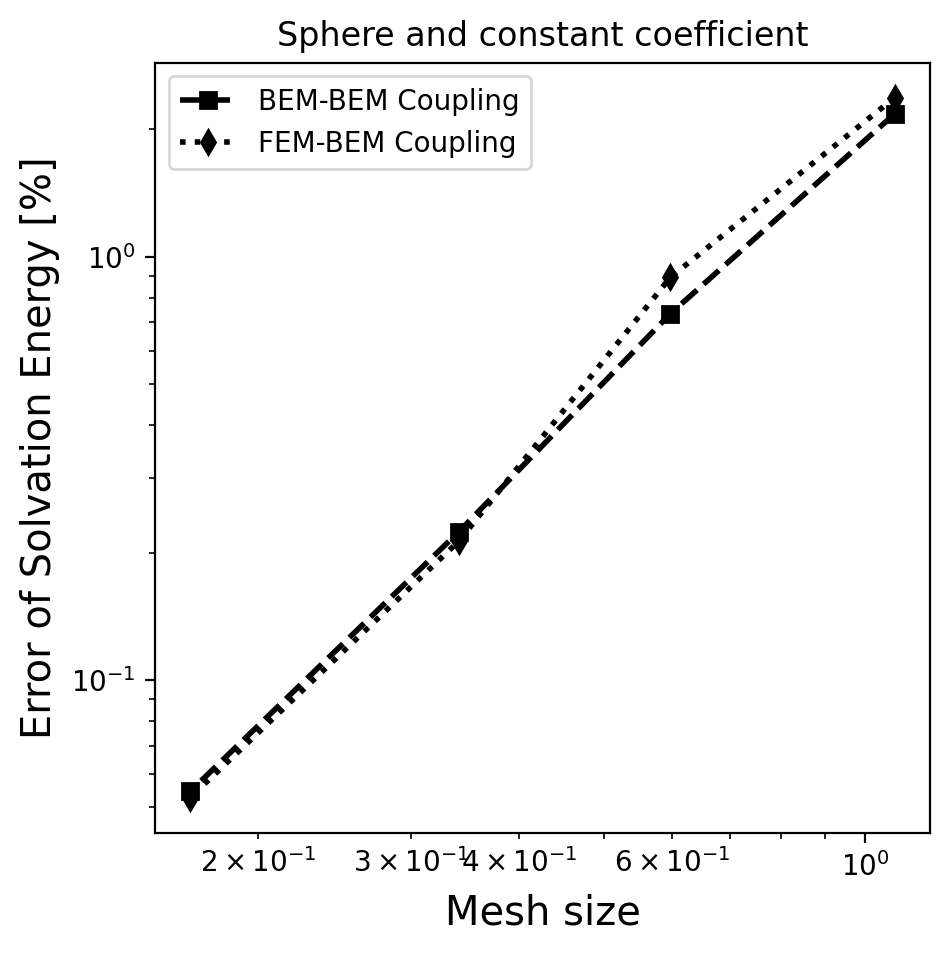
\includegraphics[width=0.45\linewidth]{DolfinX_Sphere_const_coeff_error.png}
  \caption{Error for the Kirkwood sphere.  }
  \label{fig:error_sphere}
\end{figure}

\subsection*{\sffamily \large Performance with arginine}

As a more realistic test, we assessed the performance of the FEM-BEM coupling technique against a purely BEM implementation for arginine.
The structure of arginine was taken from the protein data bank, and parameterized with the Amber\cite{ponder2003force} force field. 
We generated surface meshes containing 4.1, 6.7, 8.6, 17, and 24.5 vertices per \AA$^2$ with Nanoshaper.~\cite{decherchi2013general}
These densities correspond to a grid-scale parameter in Nanoshaper equal to 1.6, 2.0, 2.4, 3.4, and 4.0, respectively, where the grid scale is the reciprocal of the average characteristic length of the triangles.
The surface meshes were inputs to our purely BEM solver and to create the FEM mesh with pyGAMer,~\cite{lee2020open} which invoked TetGen\cite{hang2015tetgen} with a quality parameter (radius-edge ratio) of 1.0.

The solvation energy computed with the two schemes is presented in Figure \ref{fig:arg_constant_energy}, which, as expected, converges to a similar answer as the mesh is refined.
Figure \ref{fig:arg2_constant_time_iter} compares the iteration count and time-to-solution. The left plot shows that using only BEM outperforms the coupled FEM-BEM approach in terms of the iteration count. However, if we look at the total time that solvers take to obtain the solution, we can see the advantage of using the FEM-BEM coupling. The higher computational cost is caused by the need of using a hypersingular operator in the BEM formulation, and the fact that we are not using any acceleration method ($ie.$ FMM). Regardless, timings for the FEM-BEM coupling scale are much worse with size than its pure BEM counterpart, indicating that BEM-BEM coupling is better for larger problems. 
%\textcolor{red}{Chris: I thought BEM-BEM outperformed FEM-BEM in total time. Am I wrong there?} \textcolor{blue}{Michal: Not for this formulation of BEM-BEM since we have hypersingular operator. But you can see that for denser meshes we should outperform it.} 


\begin{figure}
\centering
   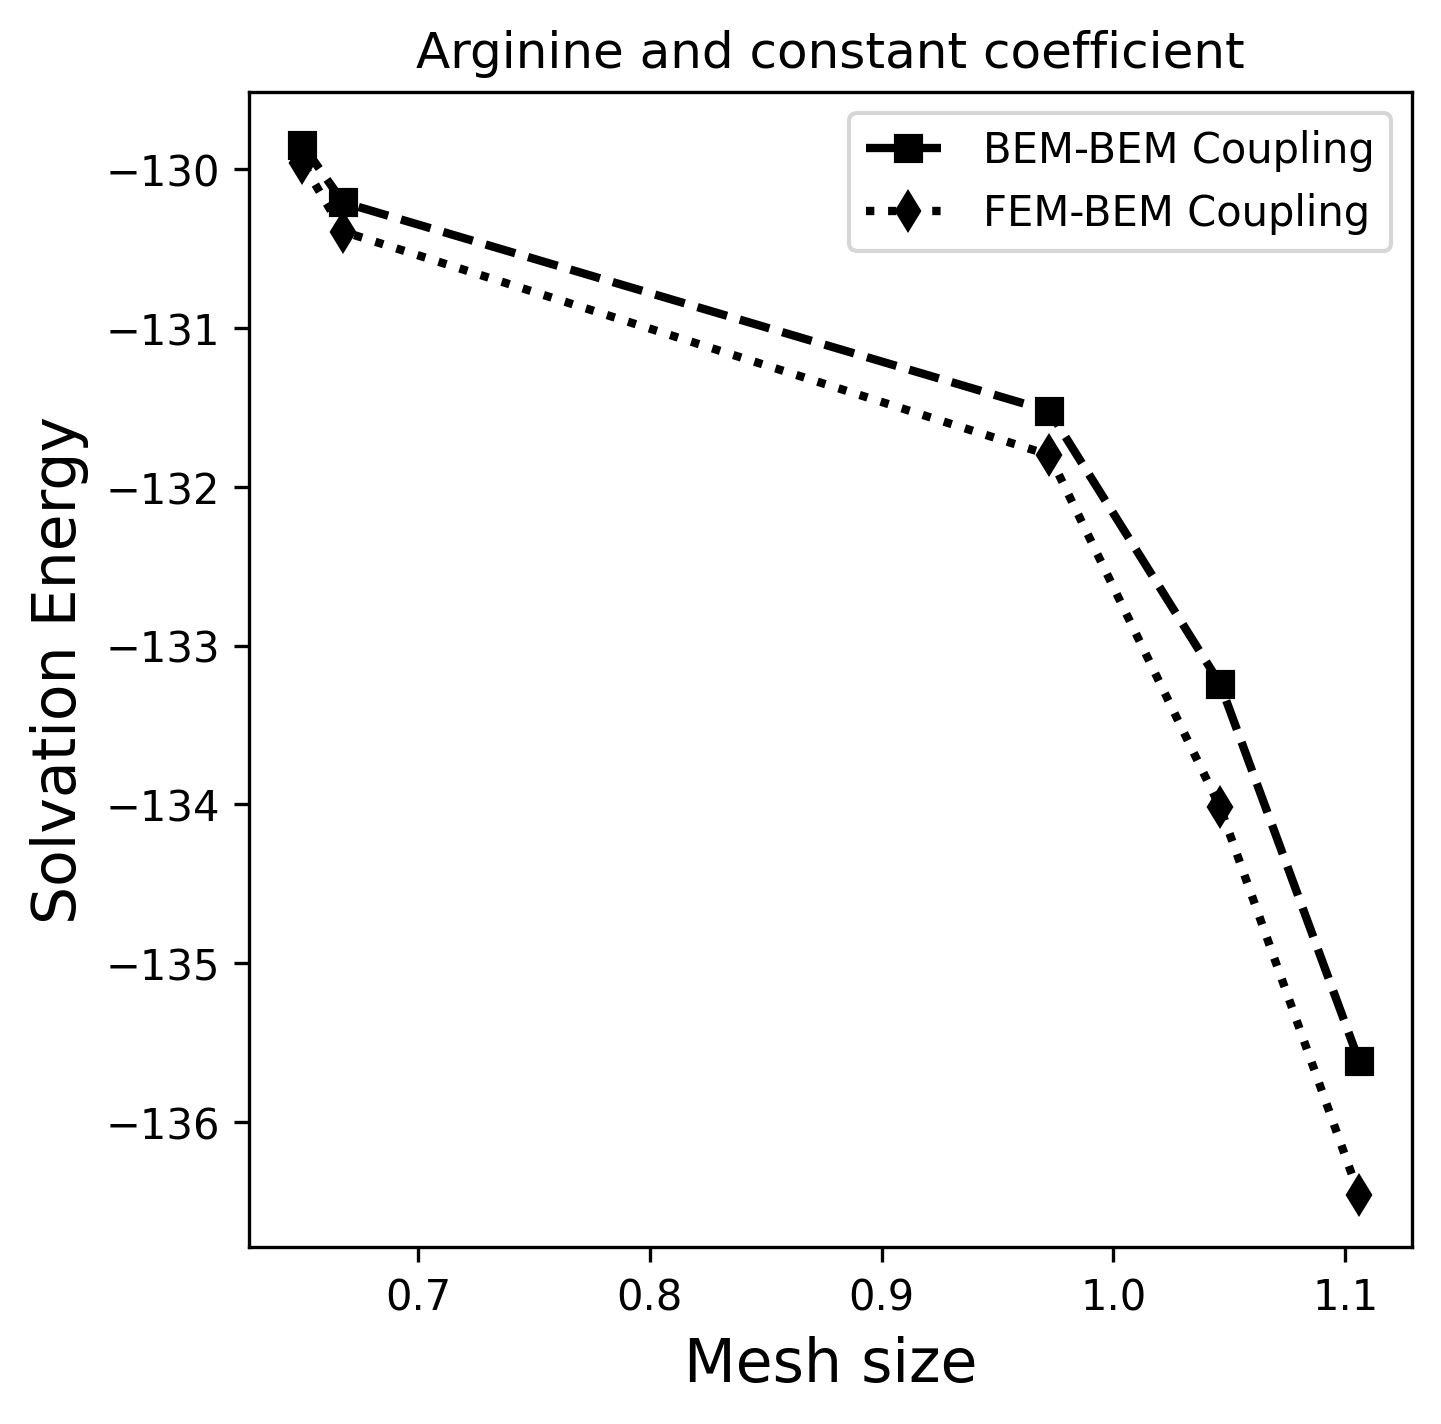
\includegraphics[width=0.45\linewidth]{DolfinX_Arginine2_const_coeff_error.png}
\caption{Solvation energy for arginine with a constant permittivity.}
\label{fig:arg_constant_energy}
\end{figure}

\begin{figure}
\centering
   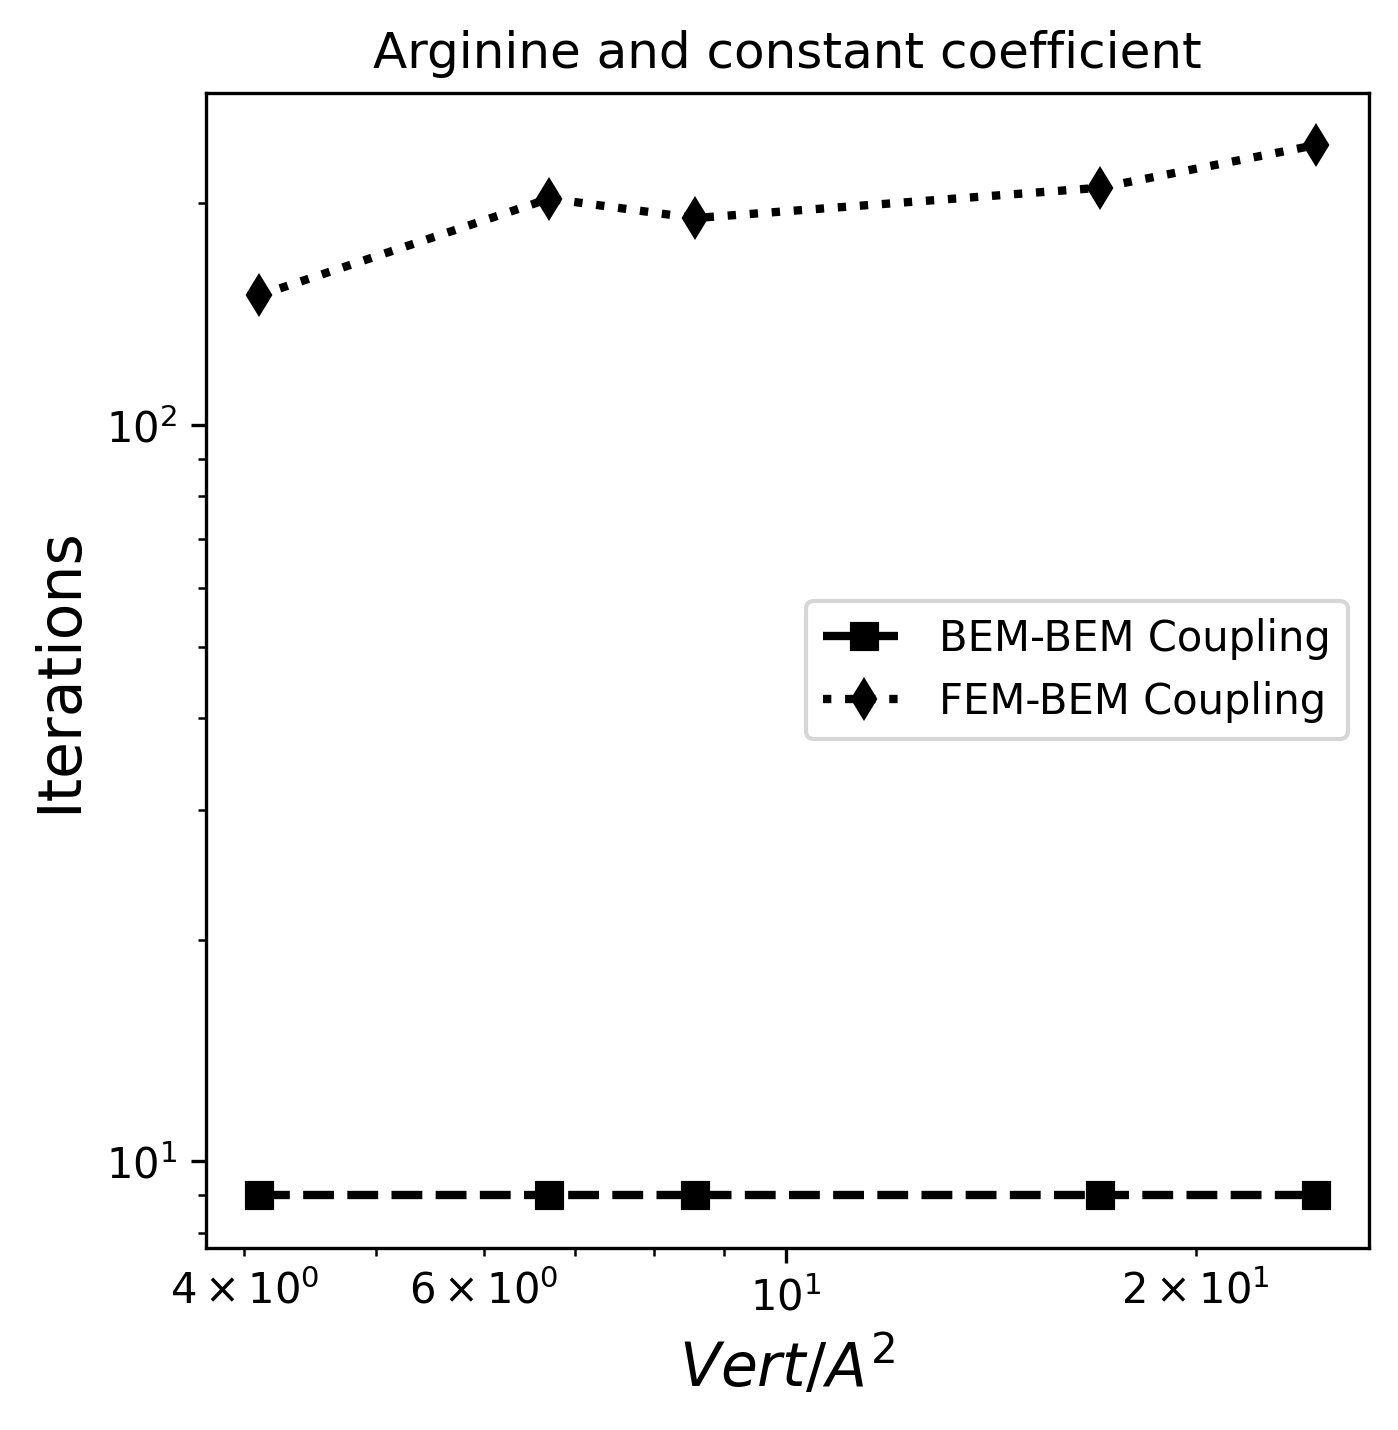
\includegraphics[width=0.45\linewidth]{DolfinX_Arginine2_const_coeff_iter.png}
  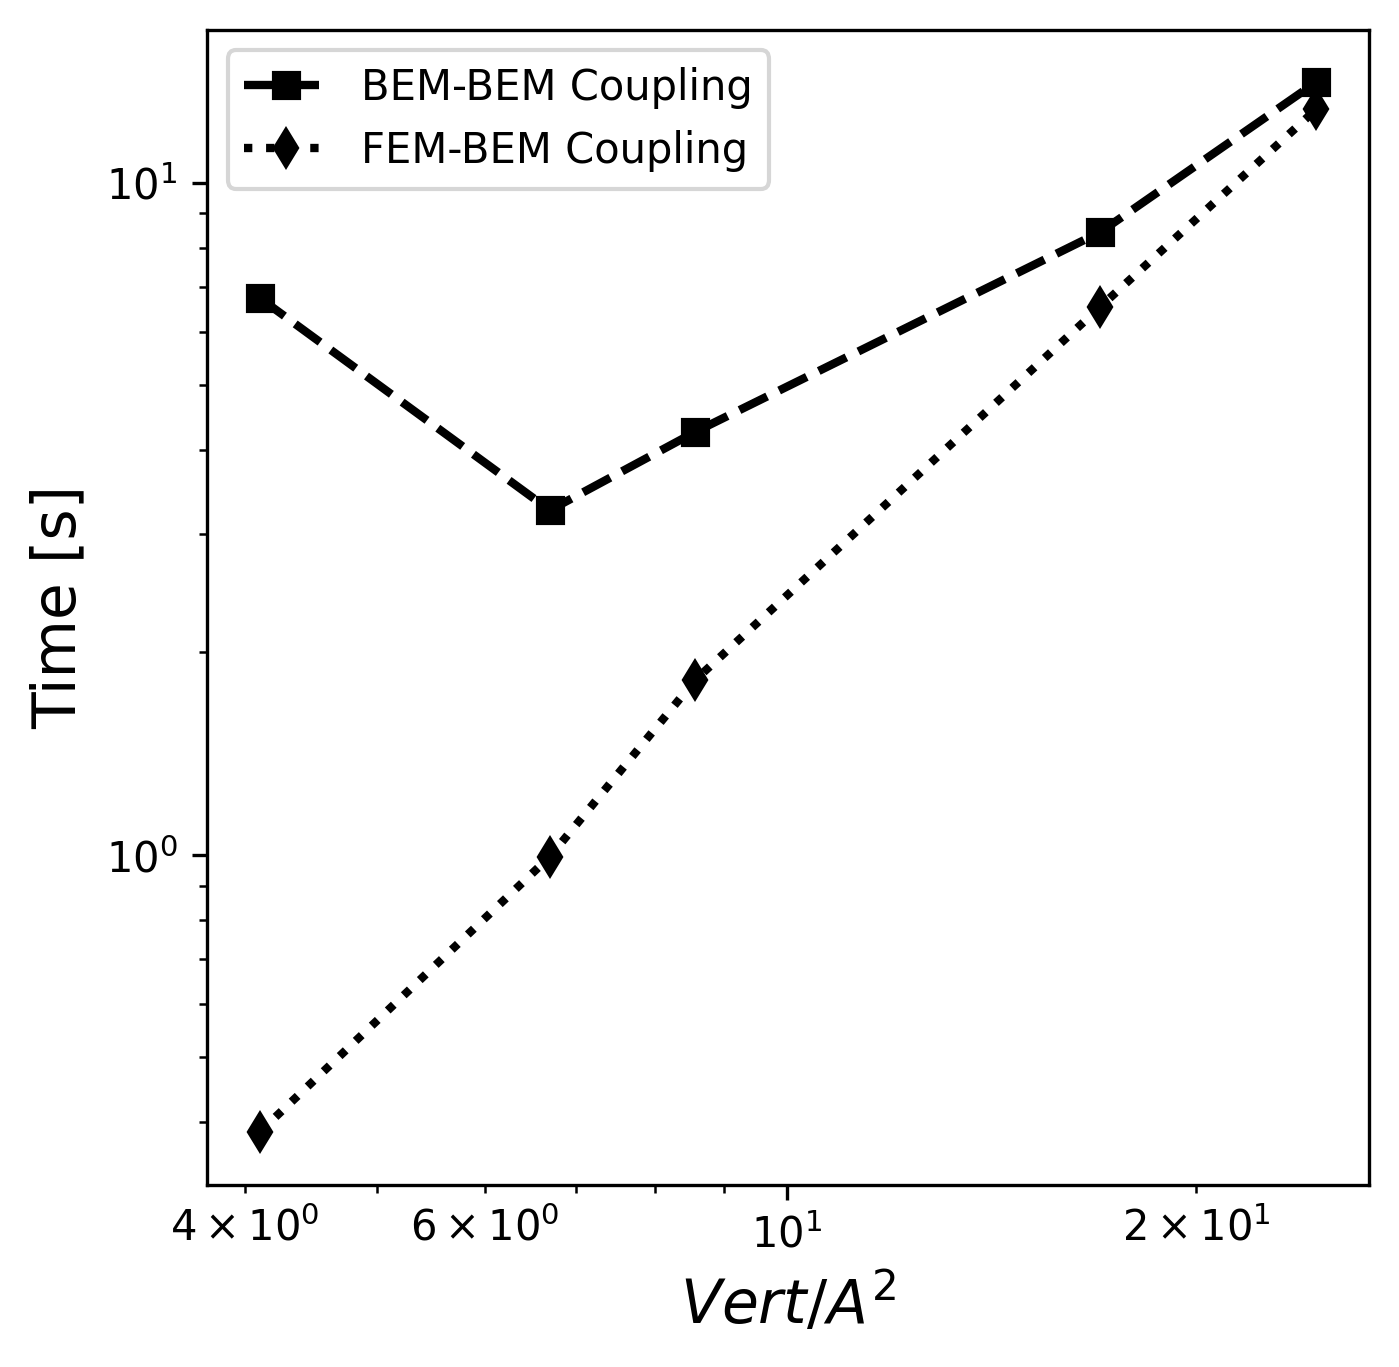
\includegraphics[width=0.45\linewidth]{DolfinX_Arginine2_const_coeff_total_time.png}
  \caption{Iteration count (left) and time-to-solution (right) for arginine with a constant permittivity.  }
\label{fig:arg2_constant_time_iter}
\end{figure}


\section*{\sffamily \Large Results with variable permittivity}

\subsection*{\sffamily \large Motivation: modeling the solute with a Gaussian-based variable permittivity}

In contrast to a purely BEM approach, FEM-BEM coupling gives the flexibility to consider space-varying field parameters. 
A popular description of the molecule is to consider a permittivity that varies like a Gaussian around each atom,\cite{grant2001smooth} which has shown enhanced accuracy in some applications, like pKa calculations.\cite{li2013dielectric}
In this setting, we define a density function $\rho$ depending on position $r$ as
%
\begin{equation}
\rho(r) := \prod_i \left(1 - \exp{\left(\frac{\|r-\mathbf{x}_i\|}{\sigma^2 R_i^2}\right)}\right)
\end{equation}
%
where the product runs over all the atoms of the solute, $R_i$ is the van der Waals radius of atom i, and we used $\sigma$=1. Then, we can compute the permittivity as
%
\begin{equation}\label{eq:varying_eps}
\epsilon := \left(1-\rho \right) \epsilon_1 + \rho\epsilon_2
\end{equation}

As $\epsilon$ is variable, Equation \eqref{eq:phic} does not have an analytical solution, and the electrostatic potential in the vacuum state has to be computed numerically.
For vacuum calculations, we considered the same distribution of $\epsilon$ inside the molecule as in the solvated case, but the solvent permittivity was set to $\epsilon_2$=2. 
Other implementations of Gaussian permittivities also modify the solute permittivity in vacuum calculations, according to a set cutoff.\cite{li2013dielectric} We did not consider a cutoff in our calculations.



\subsection*{\sffamily \large Convergence for arginine with APBS}

We used Equation \eqref{eq:varying_eps} to generate dielectric maps, which we ran on APBS~\cite{BakerETal2001} for comparison. 
We chose APBS because it provides an easy interface to control dielectric maps to ensure their agreement with the maps imposed in our FEM-BEM coupled approach.

Table \ref{table:arg_variable} shows a comparison of solvation energy computed with APBS and our FEM-BEM coupling approach. We can see that they are both converging to equivalent values, where the finest meshes agree up to 0.5\% (0.5 kcal/mol). The coarsest meshes used in both cases are within the recommended densities for accurate solvation energy simulations with constant permittivity. For example, a finite difference mesh with $h$=0.5 \AA~ or less is recommended for binding energy calculations\cite{sorensen2015comprehensive} (the result of subtracting two solvation energies), and a similar study with BEM\cite{CooperBardhanBarba2014} showed that a mesh with 2 vertices per \AA$^2$ gives acceptable results when computing binding and solvation energies. We see a jump in the solvation energy for the FEM-BEM results going from 4.1 to 6.7 vertices per \AA$^2$, but later the energy monotonically decreases, converging to a solution. This is an indication that mesh requirements for variable permittivities may be tighter than with a constant permittivity, even though the jump in dielectric constant across the molecular surface is usually smaller. 

%Figure \ref{fig:arg2_variable} contains the performance results of this test case, where we distinguish the iteration count from the calculation in dissolved and vacuum states. \textcolor{red}{Chris: if we don't include Fig. \ref{fig:arg2_variable}, we should remove this paragraph. I believe that if we show performance for fem-bem, a reviewer might be tempted to ask it for APBS too, which might be difficult.}  \textcolor{blue}{Michal: I completely agree. We were even talking about not putting them, but just for our information, we kept it for now. They weren't going to be in the final version}
\begin{table}
\centering
\begin{tabular}{c|c|c|c}
&Mesh size  & Grid points & $\Delta G_{solv}$\\
&\AA       & &  kcal/mol \\
\hline
\multirow{4}{*}{APBS}& 0.52$\times$0.52$\times$0.52 & 97$\times$97$\times$97 & -107.6186 \\ 
& 0.39$\times$0.39$\times$0.39 & 129$\times$129$\times$129 & -107.8752\\ 
&0.26$\times$0.26$\times$0.26 & 193$\times$193$\times$193& -108.3378\\ 
&0.195$\times$0.195$\times$0.195 & 257$\times$257$\times$257& -108.5837\\ 
&0.098$\times$0.098$\times$0.098 & 513$\times$513$\times$513& -108.8844\\ 
\hline
&Mesh dens. & DOFs & $\Delta G_{solv}$\\
&vert/\AA$^2$   &  &  kcal/mol \\
\hline
%%\multirow{5}{*}{Standard FEM-BEM}& 2 & -36.239\\
%    & 4.1 & 3 491 & -109.907 \\
%FEM-BEM    & 6.7  & 5 787 & -110.199 \\
%coupling    & 8.57  & 8 844 & -109.582 \\
%    & 17 & 19 911 & -109.350 \\
%    & 24.5 & 32 302 & -109.265 \\
%\hline
%\multirow{5}{*}{Standard FEM-BEM}& 2 & -36.239\\
    & 4.1 & 3 491 & -109.931 \\
FEM-BEM    & 6.7  & 5 787 & -110.237 \\
coupling    & 8.57  & 8 844 & -109.661 \\
    & 17 & 19 911 & -109.369 \\
    & 24.5 & 32 302 & -109.315 \\
\hline
\end{tabular}
\caption{Solvation energy of arginine with a Gaussian-like permittivity, computed using the FEM-BEM approach and APBS. The mesh density for FEM-BEM corresponds to the vertex density of the surface mesh used to generate the volumetric mesh.}
\label{table:arg_variable}
\end{table}

\subsection*{\sffamily \large Performance analysis for larger structures}

So far, we have only tested the FEM-BEM coupled approach with small structures. Here, we study its behaviour with larger structures to evaluate its applicability in more realistic settings, and in test cases where BEM-BEM coupling is not an alternative. Using the same Gaussian permittivity field inside the molecule, we computed the solvation free energy of protein G B1 (955 atoms, PDB code 1pgb), lysozyme (1960 atoms, PDB code 1lyz), the barnase-barstar complex (9464 atoms, PDB code 1x1u), and immunoglobulin G (20148 atoms, PDB code 1igt). All structures were parameterized with the Amber\cite{Swanson05} force field using pdb2pqr.\cite{Dolinsky04} The surface was meshed with Nanoshaper\cite{decherchi2013general} considering a grid scale of 1.5, and then used to mesh the solute region with pyGAMer\cite{lee2020open} and TetGen\cite{hang2015tetgen} with a radius-edge ratio of 1.0. Solvation free energy and timings for these runs are presented in Table \ref{table:large_variable}, showing that our FEM-BEM coupling method can reach medium-to-large-sized proteins on a workstation. For these larger structures, we enabled the FMM capabilities of Bempp-cl.

Table \ref{table:large_variable} shows that the iteration count increases with the problem size. This is expected for Johnson-N\'ed\'elec, which is the simplest coupling strategy. To isolate the effect of the increased iterations in the analysis, we separate timings in ``setup'' and ``solving'' time, where the ``setup'' time is independent of the number of iterations, and the ``solving'' time corresponds to the time spent in the GMRES solver. Then, the time-per-iteration in Table \ref{table:large_variable} only considers the ``solving'' time. Looking at the increase in degrees of freedom (DOFs), which grows equivalently for FEM and BEM, the ``setup'' time scales slightly worse than $\mathcal{O}(N^2)$, but represents the smaller fraction of the total time. On the other hand, the ``solving time per iteration'' scales closer to $\mathcal{O}(N)$, which is expected, as we are using an FMM for the BEM portion of the matrix. This is an indication that the high ``solving time'' is mainly due to the increase in iteration count, and having better-conditioned coupling methods, such as the so-called hybrid approach,\cite{betcke2022hybrid} can have a large impact on the time to solution.

Even though this scheme is capable of calculating the electrostatic potential in medium-to-large proteins, the largest test case in Table \ref{table:large_variable} (1igt) used up 30\% of the available RAM memory. 
%(\textcolor{red}{check and rewrite \textcolor{blue}{we are using around 50\% of memory}}). 
If we were aiming at larger structures, such as full viruses,\cite{MartinezETal2019,wang2021high} we would require to improve not only in the conditioning of the system but also in the optimization of our fast algorithms\cite{wang2021exafmm,kailasa2023pyexafmm} and parallelization.

\begin{table}
\centering
\resizebox{\textwidth}{!}{\begin{tabular}{c|c|c|c|c|c|c|c|c}
Molecule & FEM  & BEM &  $\Delta G_{solv}$ & Iterations & Setup Time & Solving Time & Solv. time per & Total Time \\
& DOFs & DOFs &  kcal/mol & & [sec] & [sec] & iter. [sec] & [sec] \\
\hline
% 1pgb  & 29 434 &  10 058 &  -300.389 & 613 & 89 & 410 & 0.67 & 702  \\
% 1lyz  & 56 114 & 18 606 &  -597.515 & 724 & 334 & 921  & 1.27 & 1 255   \\
% %1lyz gs3 & 257 391 & 75 048 &  -600.637 & 2 949  & 1 690 & 10 900 & 3.6 & 12 590   \\
% 1x1u & 263 181 & 81 258 &  -1 975.068 & 1 911 & 8 240 & 7 410 & 3.88 & 15 650  \\
% 1igt & 597 575 & 187 712 &   -3 279.907 & 1 974 & 40 930 & 15 600 & 7.9  &  56 530   \\
% \hline
  1pgb  & 29 434 &  10 058 &  -300.888 & 703 & 86 & 472 & 0.67 & 789  \\
 1lyz  & 56 114 & 18 606 &  -599.310 & 1 073 & 336 & 1 350  & 1.26 & 1 686   \\
 1x1u & 263 181 & 81 258 & -1 982.085 & 2 791 & 8 340 & 11 000 & 3.94 & 19 340  \\
 1igt & 597 575 & 187 712 &  -3 294.0157 & 5 366 & 41 998 & 40 100 &  7.47 & 82 098    \\
 \hline
\end{tabular}}
\caption{Results for larger structures with a variable permittivity.}
\label{table:large_variable}
\end{table}
